% fig_schematic.tex
% ------------------------------------------------------------------------------
% Figure 1 of "How Withheld Punishment Sustains Anti-Democratic Behavior in an
% Evolutionary Game": the invasion relations of the two payoff regimes.  This is
% the same TikZ code that draws the figure inside the manuscript, wrapped in a
% standalone document so that it can be compiled on its own:
%
%     pdflatex fig_schematic.tex
%
% Requires the tikz package with the arrows.meta and positioning libraries
% (standard in TeX Live).  Output: fig_schematic.pdf.
% ------------------------------------------------------------------------------
\documentclass[border=4pt]{standalone}
\usepackage{amsmath,amssymb}
\usepackage{tikz}
\usetikzlibrary{arrows.meta,positioning}
\begin{document}
\begin{minipage}{6.5in}
\begin{minipage}{0.48\linewidth}\centering
\resizebox{\linewidth}{!}{%
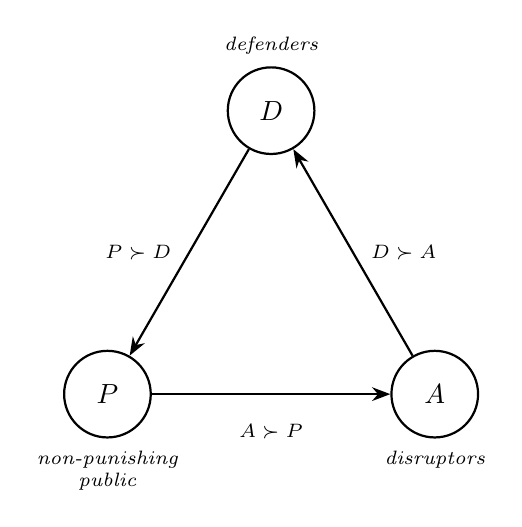
\begin{tikzpicture}[>=Stealth]
  \def\R{2.4cm}
  \node[draw, circle, thick, minimum size=11mm] (D) at (90:\R) {$D$};
  \node[draw, circle, thick, minimum size=11mm] (P) at (210:\R) {$P$};
  \node[draw, circle, thick, minimum size=11mm] (A) at (330:\R) {$A$};
  \node[font=\scriptsize\itshape,above=0.3mm of D] {defenders};
  \node[font=\scriptsize\itshape,below=0.3mm of P,align=center] {non-punishing\\public};
  \node[font=\scriptsize\itshape,below=0.3mm of A] {disruptors};
  \draw[->, thick] (D) -- node[pos=0.5, left=1mm, font=\scriptsize] {$P\succ D$} (P);
  \draw[->, thick] (P) -- node[pos=0.5, below=2.5mm, font=\scriptsize] {$A\succ P$} (A);
  \draw[->, thick] (A) -- node[pos=0.5, right=1mm, font=\scriptsize] {$D\succ A$} (D);
\end{tikzpicture}}\\[1mm]
{\footnotesize (a)}
\end{minipage}\hfill
\begin{minipage}{0.48\linewidth}\centering
\resizebox{\linewidth}{!}{%
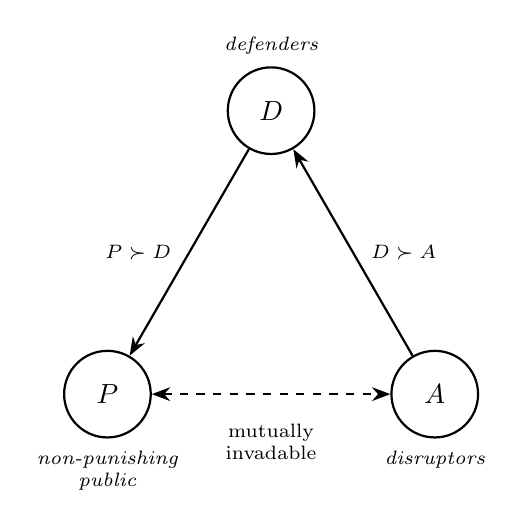
\begin{tikzpicture}[>=Stealth]
  \def\R{2.4cm}
  \node[draw, circle, thick, minimum size=11mm] (D) at (90:\R) {$D$};
  \node[draw, circle, thick, minimum size=11mm] (P) at (210:\R) {$P$};
  \node[draw, circle, thick, minimum size=11mm] (A) at (330:\R) {$A$};
  \node[font=\scriptsize\itshape,above=0.3mm of D] {defenders};
  \node[font=\scriptsize\itshape,below=0.3mm of P,align=center] {non-punishing\\public};
  \node[font=\scriptsize\itshape,below=0.3mm of A] {disruptors};
  \draw[->, thick] (D) -- node[pos=0.5, left=1mm, font=\scriptsize] {$P\succ D$} (P);
  \draw[<->, thick, dashed] (P) -- node[pos=0.5, below=2.5mm, align=center, font=\scriptsize] {mutually\\invadable} (A);
  \draw[->, thick] (A) -- node[pos=0.5, right=1mm, font=\scriptsize] {$D\succ A$} (D);
\end{tikzpicture}}\\[1mm]
{\footnotesize (b)}
\end{minipage}
\end{minipage}
\end{document}
